\section{Overview about Image Morphospecie Processing (IMP)}
The IMP was constructed to process digital image. Basically, this program look like the other applications. It include the main \textbf{menu}, \textbf{toolbar}, \textbf{main windows} and \textbf{status bar} at the end of interface
\begin{figure}[h!]
\centering
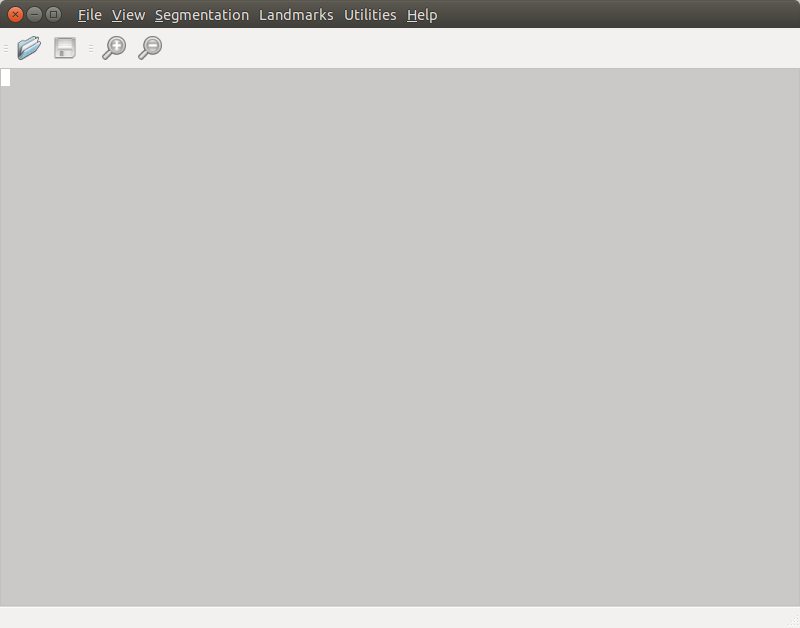
\includegraphics[scale=0.4]{images/main}
\caption{The program user interface}
\label{fig:figure_31}
\end{figure}
\subsection{Main menu}
The main menu contains all the functions of program. It was organized into the group followed the characteristics of functions. The menus \\
\textbf{File} menu contains the operations to save, open, print the image or close the program.
\subsection{Toolbar and status bar}